\chapter[Introdução]{Introdução}

\begin{comment}
Tendo em vista que já é difícil para alunos aprenderem matemática, a dificuldade só aumenta quando fala-se de alunos com Transtorno do Déficit de Atenção com Hiperatividade (TDAH) inseridos no contexto de faculdade, onde a desatenção aumenta, já que professores não estão preparados e precisam renovar seus métodos para atrair atenção dos alunos para ensinar a matéria e ainda fazer disso algo divertido para fazer com que o foco seja maior ainda. Já que aprender brincando gera melhores resultados. Segundo (Russel A. Barkley, PhD. p. iv) quem possui TDAH têm mais dificuldades que pessoas normais em ambientes que exijam mais foco, objetividade e autocontrole. Também é dito que as características principais de TDAH podem trazer diversas dificuldades no contexto escolar (George J. DuPaul, PhD e Gary Stoner, PhD. p.4).

De acordo com (George J. DuPaul, PhD e Gary Stoner, PhD. p.4) o TDAH comparado a outros problemas como autismo e depressão é um transtorno de alta incidência e se mostra presente principalmente em meninos. Por isso o foco deste estudo também será em estudantes com TDAH.
\end{comment}

O Brasil tem uma qualidade de ensino de matemática inferior a de muitos países. A Organização para a Cooperação e Desenvolvimento Econômico (OCDE) utiliza uma escala de classificação que vai de 1 a 6 para as habilidades de matemática. 70.3\% dos estudantes brasileiros estão abaixo do nível 2, o qual foi estabelecido como o mínimo para exercer a cidadania como cidadão pleno \cite{inep2015nivelcidadania}. Outros 3 fatos também contribuiram para formular a proposta deste trabalho. Um deles foi o estudo de \cite{revbibmatgam}, que é uma revisão sistemática de literatura realizada nas bases de dados Scielo Library, BIREME Biblioteca, Science Direct, ACM Library e IEEE Xplore Digital Library e nos periódicos Revista Brasileira de Informática na Educação e a Revista de Novas Tecnologias na Educação. O estudo procurou artigos que constatavam a existência de ferramentas relacionadas com gamificação e dificuldades de aprendizagem de matemática e/ou Discalculia. Por fim concluiu-se que "identifica-se a necessidade de pesquisas sobre esta temática, já que as dificuldades de aprendizagem na Matemática são frequentes
em sala de aula, e a gamificação tem-se mostrado uma ferramenta promissora nos ambientes de ensino e aprendizagem em todos os níveis de ensino" \cite{revbibmatgam}. Outro fator foi o estudo de \cite{evasaoC2} o qual diz que Cálculo 2 (C2) é uma disciplina das que mais causa a evasão dos alunos do curso de matemática noturno na UnB. Após saber deste estudo houve a comparação da ementa de C2 no curso matemática noturno e de C2 no curso de Engenharias no Gama da UnB e foi constatado que há a equivalência das disciplinas, então foram coletados e analisados as menções de Cálculo 2 (C2) da UnB dos períodos 2/2017 e 1/2018 e verificamos que a maioria das menções está concentrada no Médio (MM). Com o intuito de elevar as menções dos alunos da UnB e elevar os indicadores do conhecimento de matemática dos estudantes brasileiros 


decidiu-se fazer um jogo para celular com o intuito de inserir no ambiente dos alunos uma ferramenta a mais para ajudar os estudantes a aprender se divertindo. 

Não foi encontrado nenhum jogo de matemática para o ensino e/ou suporte de EDO. Apenas um jogo de vídeo-game que aplica ED na movimentação dos personagens (princípio da dinâmica de Newton)\cite{videoGameED}.

Avaliou-se o índice de reprovação na disciplina Cálculo 2 (C2) na UnB, nos semestres 2/2017 e 1/2018. A média foi a seguinte:

// //
O Brasil tem um dos piores índices de conhecimento em matemática \cite{indiceRuimMat}. Também tem o desânimo dos alunos e professores além da falta de estratégias inovadores por parte dos professores na hora de ensinar \cite{softwaregamificado}. Esse método de ensino tradicional, onde o professor é ativo e os alunos são apenas passivos para receber o conhecimento faz com que menos seja abstraído pelos alunos, que também precisam de práticas e um tempo de ócio criativo para abstrair e compreender o conteúdo de modo a repetir e aplicar em outras situações. Pouco foi-se encontrado de estudos na área de \textbf{matemática} + \textbf{gamificação}. A quantidade de estudos diminui quando o conteúdo de matemática é do ensino superior ao invés de ensino de matemática no ensino fundamental. 
Um outro problema é a falta de inclusão de alunos com necessidades especiais nos ambientes de sala de aula, isso deve-se à falta de preparo dos professores em sua formação \cite{matEtdah}.
// //

\begin{table}[H]
\centering
\caption{Percentual de reprovações no semestre 2/2017 e 1/2018}
\begin{tabular}{|c|c|c|}
\hline
Semestre & Total de menções & Percentual de reprovados \\ 
\toprule
2/2017 & 1164 & 32.47\% \\ 
1/2018 & 1101 & 31.88\% \\
\textbf{Total} & 2265 & 32.18\% \\
\hline
\end{tabular}
\label{tabelareprovacaoC2}
\small{Fonte: do próprio autor}
\end{table} 

A tabela mostra que aproximadamente 32\% dos alunos reprovaram de um total de 2265 alunos. 
A figura \ref{figuramencao} mostra o percentual médio das menções dos alunos da UnB de C2 nos períodos de 2/2017 e 1/2018.

\begin{figure}[H]
\centering
\caption{Percentual das menções de C2 em 2/2017 e 1/2018}
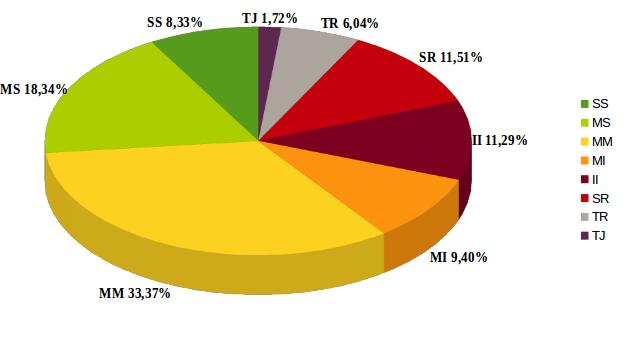
\includegraphics[scale=0.72]{figuras/grafico_media.jpg}
\label{figuramencao}
\small{Fonte: do próprio autor}
\end{figure}

O desenvolvimento do jogo é para os alunos terem uma ferramenta a mais como meio de treinamento e fixação do conhecimento para aumentarem suas menções, tendo em vista que a maior parte das menções está concentrada na menção MM, com aproximadamente 33\%. O percentual de MS é aproximadamente 18\% e SS próximo de 8\%.




Existem estudos reforçando que o jogos ajudam e aumentam as chances de aprendizado, contribuem para incluir estudantes com deficiências no meio em que estão inseridos, tornando-o mais pró ativos e melhorando suas capacidades de se articularem. 

Existem também estudos mostrando como a tecnologia da suporte para jogos na hora do ensino e ajuda na fixação do conhecimento. 

A primeira parte da metodologia seguida foi a pesquisa bibliográfica para levantar o referencial teórico a respeito do auxílio de mapas conceituais, a contribuição efetiva de jogos e seu sucesso no ensino. Já a segunda parte da metodologia foi um estudo de caso aplicado em alunos de C2 na universidade do Gama, utilizando o mapa conceitual e estatísticas levantadas do aprEnDO para avaliar o impacto do aplicativo como ferramenta de suporte ao aprendizado em EDO de 1º nível.


Dado o problema e a justificativa deste trabalho, gerou-se a questão: Como dar suporte no ensino de EDO 1ª ordem apresentados em sala de aula de forma lúdica? A partir deste questionamento, levantou-se o objetivo: desenvolver um jogo para celular Android que dê suporte ao ensino de equações diferenciais ordinárias (EDO) de 1ª ordem de forma lúdica. O jogo visa treinar os alunos a reconhecer, classificar e resolver equações presentes no dia-a-dia e no ambiente da engenharia.
O jogo conterá 2 módulos com diferentes fases de dificuldades 

As funcionalidades (\textit{features}) e a descrição granulariazada (histórias de usuários - HU) serão elencadas e descritas para que se tenha a rastreabilidade dos requisitos do jogo. 

Com o jogo pronto será aplicado em um grupo da turma de C2 no período do primeiro semestre de 2019 para que possa ser gerado dados e estatísticas para concluir se o jogo trouxe alguma eficiência no aprendizado ou não.

O capítulo 2 abordará o referencial teórico, dando ênfase nos baixos indíces de classificação do Brasil no conhecimento de matemática e apoiando a gamificação e jogos como uma prática que deixa as tarefas e atividades mais divertidas.
O capítulo 5 aborda ED para introduzir um nivelamento de conteúdo a ser abordado no jogo. O capítulo 6 explica a metodologia do trabalho. capítulo 7 explica as fases do jogo, como espera-se que ele seja jogado. capítulo 8. fala a respeito das tecnologias utilizadas para desenvolvimento e do planejamento do jogo. Capítulo 9 apresenta a conclusão do trabalho e o capítulo 10 mostra as referências do trabalho e em seguida os apêndices e anexos.